% !TEX root = ./Vorlesungsmitschrift DIFF 2.tex  
\lecture{Do 21.05. 10:15}{}
\section{Lokale Extrema unter Nebenbedingungen}
Wir betrachten folgende Situation:\\
Wir suchen Extremstellen einer Funktion \( f \) unter gewissen Nebenbedingungen \zb 
\begin{enumerate}[label=\rechtsklammer{\alph*}]
  \item\label{nebenbedingung_extremum:beispiel:mikro} (Mikro-Ökonomie) Es soll das Maximum einer Nutzenfunktion \( f(x,y)=\sqrt{xy} \), \( x>0 \), \( y>0 \), unter der Budgetbedingung \( 64=2x+8y \) bestimmt werden.
  \item\label{nebenbedingung_extremum:beispiel:geometrie} (Geometrie) Welches Dreieck kopfüber im Halbkreis hat den größten Flächeinhalt? Also \( f(b,h)=\frac{1}{2}bh \) unter dr Nebenbedingung \( \frac{1}{4}b^2+h^2=r^2 \) (Pythagoras).
  \begin{figure}[H]
    \centering
    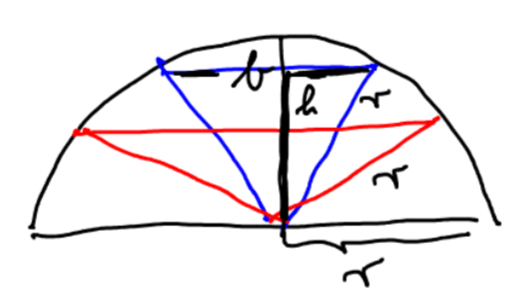
\includegraphics[width=0.4\linewidth]{figures/dreiecksmaximierung}
    \label{fig:dreiecksmaximierung}
  \end{figure}
  \item Berücksichtige, dass eine Bewegung eingeschränkt ist, \zb auf dem Innenrand einer Kugelschale (Nebenbedingung: \( x^2+y^2+z^2=r^2 \)).
\end{enumerate}
Mathematisch geht es um folgendes Problem:
\begin{definition}\label{nebenbedingung_extremum}\index{Lokales Extremum unter Nebenbedingung}
  Sei \( U\subset \reals^n \) offen, \( f\maps U\to \reals \), sei \( h\maps U\to \reals^m \). Dann sagen wir \( f \) hat in \( a\in U \) ein \emph{lokales Maximum \bzw Minimum} (Extremum) \emph{unter der Nebenbedingung} \( h(x)=0 \), wenn: \( a\in N_h(0) \) und es eine Umgebung \( U_0 \) von \( a \) gibt \sd \( f(a)\geq f(x) \) \bzw \( f(a)\leq f(x) \) \tforall \( x\in U_0 \cap N_h(0) \).
\end{definition}
In einfachen Fällen kann man die Nebenbedingung direkt auflösen und die (\ref{satz_von_der_impliziten_funktion:hoehenlinie_folgerung}) Funktion einsetzen, \zb in \ref{nebenbedingung_extremum:beispiel:mikro}
\begin{equation*}
  y=8-\frac{1}{4}x\qquad f(x,8-\quot{1}{4}x)=\sqrt{x(8-\quot{x}{4})}.
\end{equation*}
Allgemeiner: Sei \( f \), \( h \) wie in \ref{nebenbedingung_extremum} und zudem \( f \) differenzierbar und \( h\maps U\to \reals^m \), \( U\subset \reals^{n-m}\times \reals^m \), erfülle in \( a=(a_1,a_2)\in N_h(0) \) die Bedingungen des Satzes über implizite Funktionen. Also gibt es Umgebungen \( V_1 \) von \( a_1 \) und \( V_2 \) von \( a_2 \) und eine stetig differenzierbare Funktion \( g\maps V_1\to V_2 \) \sd \( N_h(0)\cap V_1\times V_2=\Set{(u,g(u))|u\in V_1} \). Also besitzt in diesem Fall \( f \) eine lokales Extremum in \( a \) unter der Nebenbedingung \( h=0 \) genau dann, wenn \( u\mapsto f(u,g(u)) \) ein lokales Extremum in \( a_1 \) besitzt.

Dies führt zur sogenannten 
\begin{satz}[Lagrange-Multiplikator-Regel]
  Sei \( f\maps U\to \reals \), \( U\subset \reals^n \) offen, in \( a\in U \) differenzierbar. Sei \( h\maps U\to \reals^m \) stetig differenzierbar, \( m<n \). Es sei \( \rang-{\totalderivative{h}(a)}=m \).

  Es besitze \( f \) in \( a \) unter der Nebenbedingung \( h(x)=0 \) ein lokales Extremum. Dann gibt es \( \lambda_1,\dotsc,\lambda_m\in \reals \) (\emph{Lagrange-Multiplikatoren}), \sd 
  \begin{equation*}
    \grad{f(a)}=\lambda_1 \grad{h_1(a)}+\dotsb+\lambda_m \grad{h_m(a)}.
  \end{equation*}
\end{satz}
\begin{proof}
  Sei \obda \( U=U_1\times U_2 \) mit \( U_1\subset \reals^{n-m} \), \( U_2\subset \reals^m \), \( a=(a_1,a_2)\in U_1\times U_2 \), (Notation \( (x,y)\in U_1\times U_2 \)) und \( \totalderivative{h}(x,y)=(D_1h(x,y) \quad  \braceannotate{\mathclap{\in \sqmatrices{m}{\reals}}}{D_2 h(x,y)})\vphantom{\underbrace{D_2 h(x,y)}_{\in \sqmatrices{m}{\reals}}} \) mit \( D_2h(a_1,a_2) \) invertierbar.
    
  \thref{satz_von_der_impliziten_funktion} \timplies \texists  \( V_1 \) offene Umgebung von \( a_1 \), \( V_2 \) offene Umgebung von \( a_2 \), \( g\maps V_1\to \reals^m \) stetig differenzierbar, \( g(V_1)\subset V_2 \), \( \totalderivative{g}(x)=-\inverse{D_2 h(x,g(x)) }\matrixmult D_1 h(x,g(x))\) und 
  \begin{equation*}
    N_h(0)\cap V_1\times V_2=\Set{(x,g(x))|x\in V_1}.
  \end{equation*}
  \( a \) ist lokale Extremstelle von \( f  \) unter der Nebenbedingung \( h(x)=0 \) \timplies \( a_1 \) ist lokale Extremstelle von
  \begin{equation*}
    V_1\ni u\mapsto f(u,g(u))=f\circ \begin{pNiceMatrix} \Id \\ g \end{pNiceMatrix}(u)
  \end{equation*}
  \timplies (Kettenregel und \ref{extremum_notwendige_bedingung})
  \begin{align*}
    &0\begin{aligned}[t]
      &=D{f\circ \begin{pNiceMatrix} \Id \\ g \end{pNiceMatrix}}(a_1)\\
      &=\totalderivative{f}(a_1,g(a_1))\matrixmult \begin{pNiceMatrix} \mathds{1}_{n-m} \\ \totalderivative{g} \end{pNiceMatrix}(a_1)\\
      &=D_1 f(a_1,a_2)-\braceannotate{(1\times m)\text{ mal }(m\times m)=(1\times m)\defines (\lambda_1,\dotsc,\lambda_m)}{D_2  f(a_1,a_2)\matrixmult \inverse{D_2 h(a_1,a_2)}}\matrixmult D_1 h(a_1,a_2)\vphantom{\underbrace{M}_{M}}
    \end{aligned}\\
    \implies &D_1 f(a)\begin{aligned}[t]
      &=(\lambda_1,\dotsc,\lambda_m )\matrixmult D_1 h(a)\\
      &=(\lambda_1,\dotsc,\lambda_m)\matrixmult \begin{pNiceMatrix} \partial_1 h_1 &  \Cdots  & \partial_{n-m}h_1 \\ \Vdots &  & \Vdots \\ \partial_1 h_m & \Cdots & \partial_{n-m} h_m \end{pNiceMatrix}(a)\\
      &=\p*{ \sum_{j=1}^{m}\lambda_j \partial_1 h_j, \sum_{j=1}^{m}\lambda_j \partial_2 h_j,\dotsc,\sum_{j=1}^{mm}\lambda_j \partial_{n-m}h_j }\\
      &=\sum_{j=1}^{m}\lambda_j D_1 h_j(a).
    \end{aligned}
  \end{align*}
  Gleichzeitig gilt (Definition der \( \lambda_j \))
  \begin{equation}
    D_2 f(a_1,a_2)\matrixmult\inverse{D_j h(a_1,a_2)}\defines (\lambda_1,\dotsc,\lambda_m),
  \end{equation}
  also (wie oben)
  \begin{align*}
    &D_2 f(a_1,a_2)=(\lambda_1,\dotsc,\lambda_m)\matrixmult D_2h(a)=\sum_{j=1}^{m}\lambda_j D_2 h_j(a)\\
    \implies &\begin{pNiceMatrix} D_1 f(a) & D_2 f(a) \end{pNiceMatrix}= \sum_{j=1}^{m} \lambda_j \begin{pNiceMatrix} D_1 h_j(a) & D_2 h_j(a) \end{pNiceMatrix}.
  \end{align*}
\end{proof}
Wir nutzt man diesen Satz zur Lösung von Problemen wie oben?
\begin{bemerkung}
  Unter Voraussetzungen an \( f \) und \( h \) wie oben betrachte das Gleichungssystem 
  \begin{gather}
    \tag{\( * \)}\label{eq:lagrange_multiplikatoren_gleichungssystem}\left.\begin{aligned}
      \partial_{\textcolor{blue}{1}}f(a)+\lambda_1\partial_{\textcolor{blue}{1}} h_1(a)+\dotsb+\lambda_m \partial_{\textcolor{blue}{1}} h_m(a)&=0\\
      \partial_{\textcolor{blue}{2}}f(a)+\lambda_1\partial_{\textcolor{blue}{2}} h_1(a)+\dotsb+\lambda_m \partial_{\textcolor{blue}{2}} h_m(a)&=0\\
      &\vdots\\
      \partial_{\textcolor{blue}{n}}f(a)+\lambda_1\partial_{\textcolor{blue}{n}} h_1(a)+\dotsb+\lambda_m \partial_{\textcolor{blue}{n}} h_m(a)&=0\\
      h_1(a)&=0\\
      &\vdots\\
      h_m(a)&=0
    \end{aligned}\right\}
  \end{gather}
  \eqref{eq:lagrange_multiplikatoren_gleichungssystem} ist gleichbedeutend mit
  \begin{equation*}
    \tag{\( ** \)} \label{eq:lagrange_multiplikatoren_kompakt}\totalderivative{f}(a)=0,
  \end{equation*}
  wenn \( F(a,\lambda)=f(a)+\sum_{j=1}^{m}\lambda_j h_j(a) \), denn \( D_1 F=0 \) liefert die ersten \( n \) Zeilen von \eqref{eq:lagrange_multiplikatoren_gleichungssystem}, \( D_2 F=0 \) lieft die letzten \( m \) Zeilen von \eqref{eq:lagrange_multiplikatoren_gleichungssystem}.

  Man versucht dann \eqref{eq:lagrange_multiplikatoren_gleichungssystem} oder \eqref{eq:lagrange_multiplikatoren_kompakt} zu lösen.
\end{bemerkung}
\begin{beispiele*}
  \begin{enumerate}
    \item Zunächst \ref{nebenbedingung_extremum:beispiel:geometrie} von oben. \( f\maps \reals_{>0}\times \reals_{>0}\to \reals \), \( f(b,h)=\frac{1}{2}bh \), \( H(b,h)=\frac{1}{4}b^2+h^2-r^2 \). \( a=(b,h) \). \( \totalderivative{f}(a)=\p*{ \frac{1}{2}h,\frac{1}{2}b } \), \( DH(a)=\p*{ \frac{1}{2}b, 2h } \). \( h>0 \) \timplies die Voraussetzungen des Satzes sind erfüllt.
    \begin{align*}
      \tag{\(*\)}&\left.\begin{aligned}
        \partial_1 f(a)+\lambda \partial_1 H(a)=\frac{1}{2}h+\frac{1}{2}b&\needed{=}0\\
        \partial_2 f(a)+\lambda\partial_2 H(a)=\frac{1}{2}b+\lambda 2H&\needed{=}0\\
        H(a)=\frac{1}{4}b^2+h^2-r^2&=0
      \end{aligned}\right\}\\
      \implies &\lambda=-\quot{b}{4h}\quad h=\quot{b^2}{4h} \implies 4h^2=b^2\\
      \underset{\text{3.\ Zeile}}{\implies} &\frac{1}{2}b^2=r^2\implies b=\sqrt{2}\quad h=\frac{1}{\sqrt{2}r}.
    \end{align*}
    \begin{figure}[H]
      \centering
      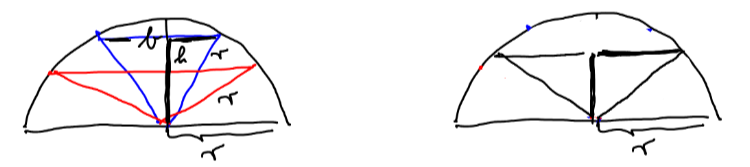
\includegraphics[width=0.5\linewidth]{figures/dreiecksmaximierung_antwort}
      \label{fig:dreiecksmaximierung_antwort}
    \end{figure}
    Der Flächeninhalt wird maximal \( \quot{1}{2}r^2 \), denn für \( b\goesto 0 \) (spitzerwerdendes Dreieck), strebt \( f\goesto 0 \), ebenso für \( h\goesto 0 \) (breiterwerdendes Dreieck).
    \item Sei \( A\in \sqmatrices{n}{\reals} \) symmetrisch. Sei \( f(x)\definedas \scalarproduct{x}{Ax} \) die zugehörige quadratische Form. Gesucht: Extrema von \( f \) unter der Nebenbedingung \( h(x)=\norm{x}_E^2-1=0 \). \( \totalderivative{h}(x)=2x\neq 0 \) \tforall \( x \) in \( N_h(0) \). Wir können also unseren Satz anwenden
    \begin{align*}
      \totalderivative{f}(a)=2A\matrixmult a\\
      \tag{\(*\)} 2A\matrixmult a+\lambda 2a\needed{=}0
    \end{align*}
    und \( \norm{a}_E=1 \). Das heißt notwendig für das Vorliegen einer Extremstelle ist, dass \( a \) Eigenvektor ist. Da \( A \) symmetrisch, ist \( A \) diagonalisierbar \timplies \texists  Eigenvektoren \( v_1,\dotsc, v_n \). Wegen \( f(v_j)=\scalarproduct{v_j}{A v_j}=\lambda_j \) Eigenwert folgt: \( f \) wird maximiert von normierten Eigenvektoren zum größten Eigenwert und minimiert von denen zum kleinsten Eigenwert.
    \item Gesucht ist der Punkt in der Ebene
    \begin{equation*}
      E=\Set{\transpose-{(x_1,x_2,x_3)}\in \reals^3|x_1+x_2-x_3=0},
    \end{equation*}
    der von Punkt \( \transpose-{(1,0,0)} \) den kleinsten Abstand hat. Da \( \Set{\transpose-{(1,0,0)}} \) kompakt ist und \( E \) abgeschlossen, gibt es einen solchen (\vgl unser Beispiel nach \thref{funktion_von_kompaktem_metrischen_raum_zu_r_kriegt_min_max}). Wir wollen also \( f(x)=\norm{x-e_1}_E^2 \) minimieren unter der Neben-Bedingung \( h(x)=x_1+x_2-x_2=0 \).

    \( \totalderivative{h}(a)=\begin{pNiceMatrix} 1 & 1 & -1 \end{pNiceMatrix} \) hat maximalen Rang (\( 1 \)) \dh jeder gesuchte Punkt \( a  \) muss erfüllen
      \begin{align*}
        2(a_1-1)+\lambda&=0\\
        2a_2+\lambda&=0\\
        2a_3-\lambda&=0\\
        a_1+a_2-a_3&=0,
      \end{align*}
    also ist \( a=\begin{pNiceMatrix} \quot{2}{3} & -\quot{1}{3} & \quot{1}{3} \end{pNiceMatrix} \) der einzige Kandidat für ein Extremum. Da es ein Minimum gibt, muss \( a \) dieses sein.
    \end{enumerate}
\end{beispiele*}
\section{Höhere Ableitungen, Taylorformel}
Ist \( f\maps U\to \reals^m \), \( U\subset \reals^n \) offen, stetig differenzierbar, kann man sich fragen, obe auch die Ableitung \( U\ni x\mapsto \totalderivative{f}(x) \) als Funktion \( \totalderivative{f}\maps U\to \matrices{m}{n}{\reals} \) wieder differenzierbar ist (in \( a \), auf ganz \( U \), auf \( V\subset U \) \dots), also ob es eine \emph{lineare} Abbildung \( A\maps \reals^n\to \matrices{m}{n}{\reals} \) gibt, \sd 
\begin{equation*}
  \totalderivative{f}(a+h)=\totalderivative{f}(a)+A(h)*\underline{R}_a^{\totalderivative{f}}(h)
\end{equation*}
mit \( \frac{\underline{R}_a^{\totalderivative{f}}(h)}{\norm{h}}\goesto 0 \) wenn \( h\goesto 0 \). Hier ist \( \underline{R}_a^{\totalderivative{f}}\maps B_{\delta}(0)\to \matrices{m}{n}{\reals} \). 

Benennt man \( \totalderivative{f}\defines g \) sieht man schnell, dass alle Sätze über differenzierbare Abbildungen natürlich auf für \( g \) gelten, insbesondere die Eindeutigkeit der Abbildung, wenn sie existiert, Kettenregel \etc. Nur kann man, wenn man nicht den Raum \( \matrices{m}{n}{\reals} \) mit \( \reals^{m\cdot n} \), die Ausdrücke im Allgem  einen mehr so leicht hinschreiben, etwa \( A(h) \) als Produkt einer Matrix mit dem Vektor \( h \).

Ist \( m=1 \) oder betrachtet man nur die Komponentenfunktionen einer \( \reals^m \)-wertigen Funktion, sieht man jedoch:
\begin{equation*}
  g\definedas \totalderivative{f}\maps U\to \matrices{1}{n}{\reals}
\end{equation*}
nimmt Werte in den \( 1\times n \)-Matrizen an, identifiziert man nun \( \matrices{1}{n}{\reals}\simeq \reals^n \) (Spaltenvektor), hat man es mit einer Funktion \( g\maps U \to \reals^n \) zu tun.

Einen \emph{Kandidaten} für \( \totalderivative{g}(a) \) findet man wieder über die partiellen Ableitungen
\begin{equation}
  \begin{pNiceMatrix} \partial_1 g(a) & \Cdots & \partial_n g(a) \end{pNiceMatrix}\in \sqmatrices{n}{\reals}
\end{equation}
und
\begin{equation*}
  g(x)=\begin{pNiceMatrix} \partial_1 f(x) \\ \Vdots \\ \partial_n f(x) \end{pNiceMatrix}
\end{equation*}
(wenn sie existieren). Insgesamt also
\begin{equation*}
  \begin{pNiceMatrix}
    \partial_1^2 f(a) & \partial_2 \partial_1 (a) & \Cdots & \partial_n \partial_1 f(a) \\
    \partial_1\partial_2 f(a) & \partial_2^2 (a) & \Cdots & \partial_n \partial_2 f(a) \\
    \Vdots & & & \Vdots\\
    \partial_1 \partial_n f(a) & \partial_2 \partial_n f(a) & \Cdots & \partial_n^2 f(a)
  \end{pNiceMatrix}\defines A
\end{equation*}
mit der Notation \( \partial_j \partial_i f(a)=\partial_j g_i(a)=\partial_j(\partial_i f)(a) \) und \( \partial_j^2=\partial_j \partial_j \).

Dann berechnet man den Rest wie üblich:
\begin{equation*}
  g(a+h)=g(a)+A\matrixmult h+ \underline{R}_a^g(h)
\end{equation*}
und überprüft, ob \( \frac{\underline{R}_a^g(h)}{\norm{h}}\goesto 0 \) für \( h\goesto 0 \).

Oder man überprüft, ob die partiellen Ableitungen stetig sind. Wenn ja, folgt die Differenzierbarkeit von \( \totalderivative{f} \) aus \thref{stetige_partielle_zu_ableitung}.

Wenn nein, muss man prüfen, ob \( \underline{R}_a^g \) das richtige Verhalten bei \( 0 \) hat. Wir werden allerdings bei den sogenannten höheren Ableitungen (wie der 2.\ Ableitung oben) meist stetig differenzierbare Funktionen betrachten.

\begin{definition}\index{$k$-fache partielle Differenzierbarkeit}
  \( f\maps U\to \reals \), \( U\subset \reals^n \) offen, heißt in \( a \) \emph{\( k \)-fach partiell differenzierbar}, wenn alle partiellen Ableitungen
  \begin{equation*}
    \partial_{j_1} f(a), \partial_{j_1} \partial_{j_2} f(a),\dotsc, \partial_{j_1}\partial_{j_2}\dotsb\partial_{j_k} f(a)
  \end{equation*}
  (Notation wie oben) \( j_i\in \Set{1,\dotsc,n} \) existieren.
  \begin{achtung*}
    Beachte, dass man zur Berechnung einer partiellen Ableitung die Funktion in einer Umgebung des Punktes kennen muss. Um also etwa eine \( k \)-te partielle Ableitung von \( f \) in \( a \) zu berechnen, muss man die \( (k-1) \)-te partielle Ableitung in einer Umgebung von \( a \) kennen.
  \end{achtung*}
  Ist \( f \) auf \( U \) \( k \)-fach partiell differenzierbar und sind alle partiellen Ableitungen der Ordnung \( \leq k \) stetig, so heißt \( f \) \emph{\( k \)-fach stetig partiell differenzierbar}.
\end{definition}
\begin{beispiel*}
  \( f(x_1,\dotsc,x_4)=x_1^3+x_2^2x_3-3x_4x_2 \). \( \partial_1^2 f(x)=6x_1 \), \( \partial_2^2 \partial_4 f(x)=\partial_2^2(-3x_2)=0 \),
  \begin{equation*}
    \partial_2 \partial_4 \partial_3 f(x)=\partial_2 \partial_4 (2x_2 x_3-3x_4)=\partial_2 (-3x_4)=0.
  \end{equation*}
  Dass die beiden letzt genannten Ableitungen gleich sind, ist kein Zufall:
\end{beispiel*}
\begin{satz}[Satz von Schwarz]\label{schwarzscher_satz}\index{Satz von Schwarz}
  Sei \( f\maps U\to \reals \), \( U\subset \reals^n \), zweimal stetig partiell differenzierbar. Dann gilt für alle \( a\in U \) und alle \( i,j\in \Set{1,\dotsc,n} \)
  \begin{equation*}
    \partial_j \partial_i f(a)=\partial_i \partial_j f(a).
  \end{equation*}
\end{satz}
\begin{proof}
  Sei \obda \( n=2 \), \( a=(a_1,a_2) \). \texists \( \delta>0 \) \sd \( B_{\delta}(a_1)\times \explain{\text{Intervall!}}{B_{\delta}(a_2)}\subset U \). Setze zu \( y\in B_\delta(a_2) \)
  \begin{equation*}
    F_y\maps B_\delta(a_1)\to \reals\qquad F_y(x)=f(x,y)-f(x,a_2).
  \end{equation*}
  MWS \timplies \texists  \( \zeta\in B_\delta(a_1)=\ointerval{a_1-\delta}{a_1+\delta} \) und zwar zwischen \( a_1 \) und \( x \) \sd 
  \begin{equation*}
    F_y(x)-F_y(a_1)=F_y'(\zeta)(x-a_1).
  \end{equation*}
  Es ist \( F_y'(\zeta)=\partial_1 f(\zeta,y)-\partial_1 f(\zeta,a_2) \). Betrachte die Funktion \( B_\delta(a_2)\ni y\mapsto \partial_1 f(\zeta,y) \). MWS \timplies \texists \( \eta\in B_\delta(a_2)=\ointerval{a_2-\delta}{a_2+\delta} \) und zwar zwischen \( a_2 \) und \( y \) \sd
  \begin{equation*}
    \partial_1 f(\zeta,y)-\partial_1 f(\zeta,a_2)=\partial_2 (\partial_1 f)(\zeta,\eta)(y-a_2).
  \end{equation*}
  Insgesamt folgt:
  \begin{equation*}
    f(x,y)-f(x,a_2)-f(a_1,y)+f(a)=\partial_2\partial_1 f(\zeta,\eta)(y-a_2)\matrixmult(x-a_1)\tag{\(*\)}.\label{eq:schwarzscher_satz:beweis:mws_1}
  \end{equation*}
  Dieselbe Konstruktion nehmen wir nun zu festen \( x\in B_\delta(a_1) \) für \( G_x(y)=f(x,y)-f(a_1,y) \) vor.

  \minisec{MWS:}
  \texists \( \tilde{\eta}\in \ointerval{a_2-\delta}{a_2+\delta} \) zwischen \( a_2 \) und \( y \) \sd \( G_x(y)-G_x(a_2)=G'x(\eta)(y-a_2) \). Es ist \( G_x'(\tilde{\eta})=\partial_2 f(x,\tilde{\eta})-\partial_2 f(a_1,\tilde{\eta}) \).

  \minisec{MWS:} 
  \texists \( \tilde{\zeta}\in \ointerval{a_1-\delta}{a_1+\delta} \) zwischen \( a_1  \) und \( x \) \sd\( \partial_2 f(x,\tilde{\eta})-\partial_2(a_1,\tilde{\eta})=\partial_1(\partial_2 f)(\tilde{\zeta},\tilde{\eta})(x-a_1) \).
  \begin{equation}
    f(x,y)-f(a_1,y)-f(x,a_2)+f(a)=\partial_1 \partial_2 f(\tilde{\zeta},\tilde{\eta})(y-a_2)\matrixmult(x-a_1)\tag{\(**\)}.\label{eq:schwarzscher_satz:beweis:mws_2}
  \end{equation}
  Aus \eqref{eq:schwarzscher_satz:beweis:mws_1} und \eqref{eq:schwarzscher_satz:beweis:mws_2} folgt für \( x\neq a_1 \), \( y\neq a_2 \)
  \begin{equation*}
    \partial_2 \partial_1 f(\tilde{\zeta},\tilde{\eta})=\partial_1 \partial_2 f(\zeta,\eta),
  \end{equation*}
  mit \( \zeta,\tilde{\zeta} \) zwischen \( a_1 \) und \( x \) und \( \eta,\tilde{\eta} \) zwischen \( a_2  \) und \( y \).

  Grenzübergang \( x\goesto a_1 \) und \( y\goesto a_2 \) liefert wegen der Stetigkeit von \( \partial_2\partial_1 f \) und \( \partial_1 \partial_2  \) die \Beh.
\end{proof}
\begin{antibeispiel*}
  \begin{equation*}
    f(x,y)=\begin{cases}
      xy\frac{x^2-y^2}{x^2+y^2}&(x,y)\neq (0,0)\\
      0 &(x,y)=(0,0)
    \end{cases}
  \end{equation*}
  Es gilt \( \partial_2 \partial_1 f(0,0)\neq \partial_1 \partial_2 f(0,0) \). Denn partielle Ableitung in \( 0 \):
  \begin{equation*}
    \partial_1 f(0,0)=\lim_{h \goesto 0}\frac{f(h,0)-f(0,0)}{h}=0=\partial_2 f(0,0).
  \end{equation*}
  Um die zweiten Ableitungen zu bestimmen, müssen wir aber \( \partial_1 f \) auch inder Nähe der \( 0 \) kennen. Daher bestimmen wir für \( (x,y)\neq (0,0) \)
  \begin{align*}
    &\begin{aligned}[t]
      \partial_1 f(x,y)&=\frac{x^4y+4x^4y^3-y^5}{(x^2+y^2)^2}\\
      \partial_2 f(x,y)&=\frac{x^5-xy^4-4x^3y^4}{(x^2+y^2)^2}
    \end{aligned}\\
    \implies &\begin{aligned}[t]
      \partial_2 \partial_1 f(0,0)&=\lim_{h \goesto 0}\frac{1}{h}(\partial_1 f(0,h)-\partial_1f(0,0))\\
      &=\lim \frac{1}{h}(\quot{-h^5}{h^4})=-1\\
      \partial_1 \partial_2 f(0,0)&=\lim_{h \goesto 0}\frac{1}{h}(\partial_2 f(h,0)-\partial_2 f(0,0))\\
      &=\lim \frac{1}{h}(\quot{h^5}{h^4})=+1.
    \end{aligned}
  \end{align*}
\end{antibeispiel*}
\section{Der Laplace-Operator}
Sei \( f\maps U\to \reals \), \( U\subset \reals^n \) offen, zweimal partiell stetig differenzierbar. Man setzt
\begin{equation*}
  \laplaceoperator f(x)\definedas \partial_1^2 f(x)+\partial_2^2 f(x)+\dotsb+\partial_n^2 f(x)
\end{equation*}
und nennt \( \laplaceoperator=\partial_1^2+\dotsb+\partial_n^2 \) den \emph{Laplace-Operator}.
\begin{beispiele*}
  \begin{enumerate}
    \item \( h\maps \reals^n\setminus\zeroset\to \reals \), \( h(x)=f(\norm{x}_E) \) mit einer auf \( \reals\setminus \zeroset \) zweimal stetig partiell differenzierbaren Funktion \( f \).
    \begin{equation*}
      \grad{f(\norm{x}_E)}=f'(\norm{x}_E)\frac{1}{\norm{x}_E}x
    \end{equation*}
    und
    \begin{align*}
      &\partial_i\p*{f'(\norm{x}_E)\frac{1}{\norm{x}_E}x_i }=f''(\norm{x}_E)\frac{x_i}{\norm{x_i}}\cdot\frac{x_i}{\norm{x}_E}+f'(\norm{x}_E)\p*{ -\frac{1}{2}\frac{2x_i}{\sqrt{\sum x_j^2}^3}\cdot x_i +\frac{1}{x_E} }\\
      \implies &\laplaceoperator h(x)=f''(\norm{x}_E)+f'(\norm{x}_E)\frac{1}{\norm{x}_E}(n-1)
    \end{align*}
    \item In Kugelkoordinaten: Sei \( g\maps \reals_{>0}\times \reals\times\reals\to \reals^3 \)
    \begin{equation*}
      g(r,\tau,\phi)=\begin{pNiceMatrix} r\Cos{\phi} \Sin{\theta}\\ r\Sin{\phi}\Sin{\theta}\\ r\Cos{\theta} \end{pNiceMatrix}.
    \end{equation*}
    \begin{figure}[H]
      \centering
      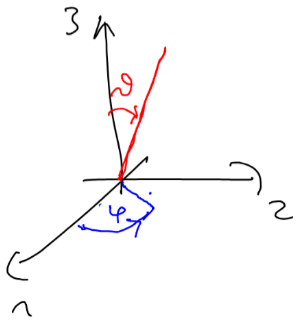
\includegraphics[width=0.5\linewidth]{figures/kugelkoordinaten}
      \label{fig:kugelkoordinaten}
    \end{figure}
    \( g \) ist zweimal stetig partiell differenzierbar.

    Sei \( f \) zweimal stetig differenzierbar auf \( \reals^3\to \reals \). \( \laplaceoperator f \) in Kugelkoordinaten bestimmen, also wenn wir \( \begin{pNiceMatrix} x \\ y \\ z \end{pNiceMatrix}=g(r,\theta,\phi) \)  schreiben. Zunächst überlegen wir, was es heißt, \( f  \) in Kugelkoordinaten zu schreiben.
    \begin{beispiel*}
      \( f(x,y,z)=xyz \).
      \begin{equation*}
        f\circ g(r,\theta,\phi)=f(r\Cos{\phi}\Sin{\theta},r\Sin{\phi}\Sin{\theta}, r\Cos{\theta})=r^3\sin^2\theta\Cos{\theta}\Cos{\phi}\Sin{\phi}\defines F(r,\theta,\phi).
      \end{equation*}
      Sodann:
      \begin{equation*}
        \totalderivative{g}(r,\theta,\phi)=\begin{pNiceMatrix}
          \Cos{\phi}\Sin{\theta}& r\Cos{\phi}\Cos{\theta} & -r\in \phi\Sin{\theta}\\
          \Sin{\phi}\Sin{\theta}& r\Sin{\phi}\Cos{\theta} & r\Cos{\phi}\Sin{\theta}\\
          \Cos{\theta} & -r\Sin{\theta}& 0
        \end{pNiceMatrix}
      \end{equation*}
      \( \Det \totalderivative{g}(r,\theta,\phi)=r^2\Sin{\theta}\) \timplies Ist \( v\neq k\pi \), \( k\in \wholes \), so ist \( g \) lokal umkehrbar mit stetig differenzierbarer Umkehrfunktion \( h\maps W\to V \) und in \( (x,y,z)\in W \) gilt
      \begin{align*}
        &f(\underbrace{x,y,z}_{=g(r,\theta,\phi)})=f\circ g\circ h(x,y,z)\defines F\circ h(x,y,z)\\
        \implies &\totalderivative{f}(x,y,z)=\explain{DF(r,\theta,\phi)}{\text{\( 1\times 3 \)-Matrix}}\matrixmult \overset{\underset{\downarrow}{\text{\( 3\times 3 \)-Matrix}}}{\underbrace{\totalderivative{h}(x,y,z)}_{=\inverse{\totalderivative{g}(r,\theta,\phi)}}}\defines \explain{\text{\( 1\times 3 \)-Matrix}}{\tilde{F}(r,\phi,\theta)}=\tilde{F}\circ h(x,y,z)\\
        \implies &(\partial_1^2+\partial_2^2+\partial_3^2)f(x,y,z)\begin{aligned}[t]
          &=\partial_1(\tilde{F}\circ h)_1 (\underbrace{x,y,z}_{\defines x})+\partial_2(\tilde{F}\circ h)_2 (x,y,z)+\partial_3(\tilde{F}\circ h)_3 (x,y,z)\\
          &=\sum_{j=1}^{3}(\partial_j \cdot \tilde{F}_j)(\underbrace{h(x)}_{\mathclap{=(r,\phi,\theta)}})\cdot\underbrace{\partial_j h_j(x)}_{\phantom{\partial_j g_j(r,\phi,\theta)}=\frac{1}{\partial_j g_j(r,\phi,\theta)}} \qquad (\text{Umkehrsatz})\\
          &=\sum_{j=1}^{3}\partial_j \tilde{F}_j(r,\theta,\phi)\cdot\frac{1}{\partial_j g_j(r,\phi,\theta)}.
        \end{aligned}
      \end{align*}
      Eine etwas längere Rechnung, bei der man \ua \( \totalderivative{g}(r,\theta,\phi) \) invertieren muss, liefert die explizite Formel für die \( \tilde{F}_j \), etwa
      \begin{equation*}
        \tilde{F}_1=\begin{pNiceMatrix} \partial_1 F & \partial_2 F & \partial_3 F \end{pNiceMatrix}\matrixmult\explain{\text{1.\ Spalte von \( \inverse{\totalderivative{g}(r,\theta,\phi)} \)}}{\begin{pNiceMatrix} \Cos{\phi}\Sin{\theta}\\ \frac{1}{r}\Cos{\phi}\Sin{\theta}\\ -\frac{1}{r}\frac{\Sin{\phi}}{\Sin{\theta}} \end{pNiceMatrix}}.
      \end{equation*}
      Von diesen berechnet man die jeweilige partielle Ableitung \( \partial_j \tilde{F}_j \) und multipliziert mit \( \frac{1}{\partial_j g_j} \).

      \zb
      \begin{align*}
        \partial_1 \tilde{F}_1&=\partial_1^2 F\cdot\Cos{\phi}\in \theta+\partial_1 \partial_2 \cdot\frac{1}{r}\Cos{\phi}\Cos{\theta}-\partial_2 F\cdot \frac{1}{r^2}\Cos{\phi}\Cos{\theta}-\partial_1 \partial_3 \cdot\frac{1}{r}\frac{\Sin{\phi}}{\Sin{\theta}}+\partial_3 F\frac{1}{r^2}\frac{\Sin{\phi}}{\Sin{\theta}}\\
        \quot{1}{\partial_1 g_1}&=\frac{1}{\Cos{\phi}\Sin{\theta}}.
      \end{align*}
      Das Ergebnis ist
      \begin{equation*}
        \frac{1}{r^2}\underset{=\partial_1}{\partial_r}(r^2\underset{=\partial_1}{\partial_r}F)+\frac{1}{r^2\Sin{\theta}}\underset{=\partial_2}{\partial_{\theta}}(\Sin{\theta}\underset{=\partial_2}{\partial_{\theta}} F)+\frac{1}{r^2\sin^2\theta}\underset{=\partial_3^2}{\partial_{\phi}^2}F.
      \end{equation*}
    \end{beispiel*}
  \end{enumerate}
\end{beispiele*}
\begin{ergaenzung*}
  \begin{figure}[H]
    \centering
    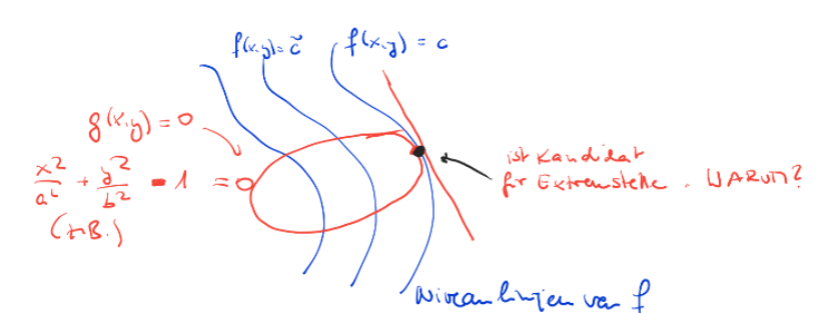
\includegraphics[width=0.9\linewidth]{lagrange_multiplikatoren_intuition}
    \label{fig:lagrange_multiplikatoren_intuition}
  \end{figure}
  Tatsache: \( \grad{h}(x,y) \) steht senkrecht auf \( h(x,y)=c \). (Der Gradient zeigt in die Richtung des stärksten Anstiegs der Funktion).
  \begin{figure}[H]
    \centering
    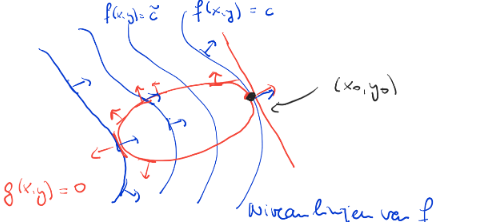
\includegraphics[width=0.9\linewidth]{lagrange_multiplikatoren_weitere_intuition}
    \label{fig:lagrange_multiplikatoren_weitere_intuition}
  \end{figure}
  Tatsache 2: Liegt in \( (x_0,y_0)\in \set{(x,y)|g(x,y)=0} \) ein Extremum von \( f \), so \texists \( \lambda\in \reals \) \sd \(\boxed{ \grad{f}(x_0,y_0)\lambda\grad{g}(x_0,y_0) }\). Tatsache 1 + 2 gleichbedeutend \( f(x,y)=c \) schmiegt sich in \( (x_0,y_0,) \) tangential an \( \set{g(x,y)=0} \) an.

  Das heißt, wenn wir das Gleichungssystem
  \begin{equation*}
    \left.\begin{aligned}
      \grad{f}(x,y)-\lambda\grad{g}(x,y&)=0\\
      g(x,y)&=0
    \end{aligned}\right\}\tag{\( * \)}\label{eq:lagrange_multiplikatoren_intuition}
  \end{equation*}
  lösen, haben wir Kandidaten für Extremstellen gefunden.
  \begin{align*}
    \eqref{eq:lagrange_multiplikatoren_intuition}\therefore \begin{aligned}[t]
      \partial_x L&=0\\
      \partial_y L&=0\\
      \partial_{\lambda} L&=0,
    \end{aligned}
  \end{align*}
  \( L \) Lagrange-Funktion.
\end{ergaenzung*}